\chapter{Resultados y conclusiones.}




\section{Estimaci\'on de par\'ametros y curva de rendimiento.}

\hspace{0.4cm} Una vez construida la base de datos, se proceder\'a a utilizar los splines de suavizado para obtener los par\'ametros necesarios para la curva de rendimientos. Recordemos que esta curva relaciona el plazo del instrumento con su rendimiento.


\hspace{0.4cm} Es importante se\~nalar que se estimar\'a una curva por cada tipo de instrumento, as\'i se obtendr\'a un curva para los TIF y una curva para los VEBONO. Por tal raz\'on a partir de la base de datos, se separar\'a los TIF de los VEBONOS, y se considerar\'an s\'olo las columnas Plazo y Rendimiento para estimar dicha curva. Seg\'un sea el caso, s\'olo considerar\'an aquellas observaciones que tengan decisi\'on 1.


\hspace{0.4cm} Aunado a cada tipo de instrumento (TIF \'o VEBONO), se considerar\'a un instrumento de otro tipo este es la letra del tesoro, este tipo de instrumento representar\'a el punto inicial la curva, cabe destacar que la letra a considerar debe ser aquella cuya fecha de operaci\'on sea la m\'as reciente con respecto a la fecha de valoraci\'on (d\'ia en que se quiere conocer los rendimientos estimados).


\hspace{0.4cm} A partir de la curva de rendimientos obtenida (Ver figura \ref{c_rend}) es posible calcular un rendimiento estimado para alg\'un tipo de instrumento a partir de su plazo, que no es m\'as que la cantidad de d\'ias que faltan por transcurrir hasta su vencimiento. Este valor es de suma importancia ya que a partir del mismo es posible calcular el precio estimado asociado a cada instrumento en un d\'ia espec\'ifico. Con lo cual es posible saber a partir de la historia (base de datos), el precio estimado de alg\'un instrumento que le interese a cierta instituci\'on y por ende saber si ese t\'itulo es rentable o no, es decir, si vale la pena invertir en el mismo o no.

\begin{figure}[h]
  \scalebox{0.40}{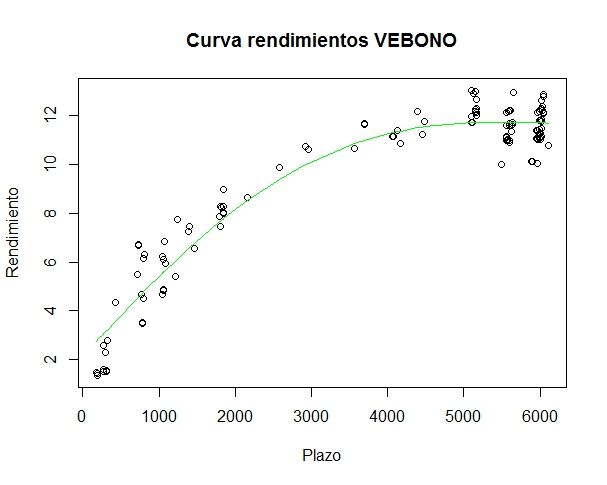
\includegraphics{images/curvarend.jpeg}}
\caption{Curva de Rendimiento.}
\label{c_rend}
\end{figure}

\hspace{0.4cm} Como se dijo anteriormente, los resultados de los precios obtenidos mediante el uso de la metodolog\'ia de splines de suavizado ser\'an comparados con los precios obtenidos a trav\'es de la metodolog\'ia de Svensson. En dicha metodolog\'ia existe un proceso de optimizaci\'on el cual permite encontrar los par\'ametros id\'oneos, de tal manera que la diferencia entre los precios promedio de cada instrumento y su precio te\'orico sea lo m\'as peque\~na posible. El proceso de esta optimizaci\'on se muestra a continuaci\'on.


%\section{Elecci\'on \'optima del par\'ametro de suavizamiento.}

\section{Proceso de Optimizaci\'on de Svensson.}


\hspace{0.4cm} Para aplicar este proceso es necesario tener una funci\'on objetivo, sobre la cual se realizar\'a el proceso de optimizaci\'on, ya sea para maximizar \'o minimizar dicha funci\'on. Dependiendo de la forma de dicha funci\'on el proceso de optimizaci\'on ser\'a lineal o no lineal. En nuestro caso particular se llevar\'a a cabo un proceso de optimizaci\'on no lineal donde se buscar\'a minimizar la funci\'on objetivo.

\vspace{0.5cm}

\hspace{0.4cm} En el c\'alculo de nuestra funci\'on objetivo inteviene el concepto de la duraci\'on de un bono \'o t\'itulo, la cu\'al es una medida del vencimiento medio ponderado de todos los flujos que paga un bono. La misma viene dada mediante la siguiente expresi\'on, \\

\begin{center}

$\displaystyle{Duracion = \frac{1+r}{r} - \frac{n(c-r)+(1+r)}{c(1+r)^{n}-(c-r)}}$

\end{center}

\vspace{0.5cm}

\newpage

\noindent donde

\begin{itemize}
  \item r es el rendimiento al vencimiento del bono durante el per\'iodo considerado.
  \item n es el n\'umero de per\'iodos que restan hasta la fecha de vencimiento del bono.
  \item c es el cup\'on del bono.
\end{itemize}


\vspace{0.5cm}

\hspace{0.4cm} As\'i nuestra funci\'on objetivo viene dada mediante la siguiente expresi\'on,\\

\begin{equation}\label{ecua2}
  f(x) = \sum_{i=1}^{n} (w_{i}\epsilon(x)_{i} )^2
\end{equation}



\vspace{0.5cm}
\noindent donde $w_{i}$ representan las ponderaciones, y se calculan mediante la siguiente expresi\'on,\\

\begin{center}

$\displaystyle{w_{i} = \frac{\frac{1}{D_{i}}}{\sum_{j=1}^{N}\frac{1}{D_{j}}}}$

\end{center}

\vspace{0.5cm}

\noindent por su parte, $\epsilon_{i}(x)= \hat{Pr}_{i}(x)-Pr_{i}$, donde $Pr_{i}$ representan los precios promedios de los t\'itulos a considerar, de entrada este es un par\'ametro \'o valor con el que se cuenta. Por otra parte $\hat{Pr}_{i}(x)$ representa los precios estimados donde $x$ es el par\'ametro que va a variar y es el valor que se quiere optimizar.

\vspace{0.5cm}

\hspace{0.4cm} Mediante la funci\'on objetivo descrita anteriormente se busca minimizar la diferencia que existe entre los precios promedios y los precios estimados, calculando un valor \'optimo del par\'ametro $x$ mediante el proceso de optimizaci\'on no lineal.

\vspace{0.5cm}

\hspace{0.4cm}El proceso de optimizaci\'on se realiz\'o mediante el software estad\'istico R, mediante el paquete ``nloptr". En este paquete, se encuentra el comando ``aulag" el cual minimiza un funci\'on objetivo y devuelve entre otros valores el par\'ametro m\'as \'optimo, que hace que la funci\'on sea m\'inima. Un ejemplo del uso de este comando se presenta acontinuaci\'on,

\vspace{0.5cm}
\begin{center}
  $ala2=auglag(1.22, fn=mifuncion, hin=res)$
\end{center}

\vspace{0.5cm}

\noindent donde el primer argumento debe ser el valor inicial del par\'ametro a optimizar, el segundo argumento ``fn" se refiere a la funci\'on que se desea optimizar, finalmente en el tercer par\'ametro ``hin" se indican las restricciones sobre el par\'ametro a optimizar, en este caso la restricci\'on establecida es que el par\'ametro sea mayor a cero.


\hspace{0.4cm} Como se observ\'o en las secciones anteriores el par\'ametro de suavizamiento fu\'e elegido mediante el m\'etodo de ensayo y error el cual no es para nada \'optimo pues a priori este m\'etodo no nos garantiza que el valor seleccionado sea el mejor, ya que se contar\'ian con una gran cantidad de posibles valores a seleccionar, con el fin  de encontrar dicho par\'ametro el procedimiento anteriormente explicado puede ser implementado. Sin embargo, al realizar este proceso, se obtienen curvas que no son para nada suaves y en ocasiones no poseen ningunas de las formas usuales de la curva de rendimientos. Esto es debido a que en este caso este proceso, var\'ia el par\'ametro de suavizamiento de tal manera que la diferencia entre el precio promedio y el precio te\'orico sea lo mas peque\~na posible y en este proceso no existe un par\'ametro que controle la forma de la curva obtenida. Por lo tanto, su aplicaci\'on presenta algunos inconvenientes.  



\hspace{0.4cm} La comparaci\'on de los precios obtenidos con la metodolog\'ia Svensson para los Tif, se presenta a continuaci\'on,

\begin{center}
\scalebox{0.90}{\begin{tabular}[t]{|c |c |c |c |c |c |r|}
\hline
T\'itulo & Precio Promedio & Precio Splines & Precio Svensson & Precio Svensson Optimizado  \\
\hline
TIF082018 & 101,00 & 107,27 & 107,35 & 100,92  \\
\hline
TIF042019 & 112,00 & 116,38 & 119,48 & 113,41  \\
\hline
TIF082019 &  110,00& 109,42 & 112,81 & 108,19 \\
\hline
TIF112020 & 130,02 & 127,62 & 130,15 & 127,28  \\
\hline
TIF022021 & 129,01 & 128,05 & 130,37 & 127,56  \\
\hline
TIF042023 & 128,10 & 132,21 & 134,03 & 130,27  \\
\hline
TIF012024 & 120,00 & 134,42 & 136,25 & 132,02 \\
\hline
TIF062025 & 124,00 & 130,44 & 131,61 & 126,85  \\
\hline
TIF012026 & 122,00 & 130,31 & 131,05 & 126,04  \\
\hline
TIF112027 & 126,52 & 132,04 & 130,75 & 125,08 \\
\hline
TIF032028 & 128,52 & 135,83 & 134,02 & 128,15  \\
\hline
TIF052028 & 128,19 & 137,56 & 131,76 & 125,88  \\
\hline
TIF032029 & 132,03 & 140,30 & 137,37 & 131,18  \\
\hline
TIF022030 & 128,52 & 142,86 & 138,91 & 132,42  \\
\hline
TIF022031 & 130,10 & 135,95 & 131,54 & 125,01  \\
\hline
TIF032031 & 128,53 & 138,30 & 133,87 & 127,30  \\
\hline
TIF022032 & 127,00 & 135,13 & 127,48 & 120,92\\
\hline
TIF032032 & 128,52 & 139,45 & 135,46 & 128,60  \\
\hline
TIF032033 & 127,01& 135,37 & 130,67 & 123,91\\
\hline
TIF052034 & 127,12 & 128,51 & 124,08 & 117,35\\
\hline
SRC & NA & 4,6224 & 5,2694 & 0,3610\\
\hline
\end{tabular}}
\end{center}

\hspace{0.4cm}La siguiente tabla muestra los resultados obtenidos para los Vebonos al d\'ia 01/03/2018,

\begin{center}
\scalebox{0.90}{\begin{tabular}[t]{|c |c |c |c |c |c |r|}
\hline
T\'itulo & Precio Promedio & Precio Splines & Precio Svensson & Precio Svensson Optimizado  \\
\hline
VEBONO072018 & 100,40 & 106,17 & 108,14 & 102,32  \\
\hline
VEBONO022019 & 106,00 & 107,75 & 111,18 & 102,75  \\
\hline
VEBONO032019 &  110,00& 113,55 & 117,10 & 108,68 \\
\hline
VEBONO012020 & 121,00 & 118,42 & 121,05 & 116,78  \\
\hline
VEBONO062020 & 127,83 & 120,97 & 122,60 & 121,85  \\
\hline
VEBONO012021 & 130,32 & 121,96 & 122,27 & 125,85  \\
\hline
VEBONO052021 & 127,00 & 122,01 & 121,72 & 127,10 \\
\hline
VEBONO122021 & 129,45 & 126,18 & 124,86 & 132,83  \\
\hline
VEBONO022022 & 129,00 & 123,15 & 121,55 & 130,09 \\
\hline
VEBONO012023 & 129,96 & 126,79 & 123,69 & 134,17 \\
\hline
VEBONO022024 & 128,00 & 128,27 & 123,88 & 134,55  \\
\hline
VEBONO022025 & 128,50 & 134,25 & 125,35 & 135,15  \\
\hline
VEBONO042028 & 129,68 & 132,08 & 127,80 & 133,37  \\
\hline
VEBONO102028 & 130,01 & 131,67 & 127,68 & 132,63  \\
\hline
VEBONO052029 & 125,03 & 131,16 & 127,26 & 131,61  \\
\hline
VEBONO102029 & 125,75 & 132,32 & 128,24 & 132,14 \\
\hline
VEBONO072030 & 130,50 & 132,44 & 127,72 & 130,89\\
\hline
VEBONO062032 & 128,53 & 128,07 & 121,73 & 123,20  \\
\hline
VEBONO072033 & 130,00& 127,31 & 120,40 & 121,26\\
\hline
VEBONO022034 & 128,02 & 126,53 & 119,49 & 120,01\\
\hline
SRC & NA & 3,5817 & 6,7379 & 0,8590\\
\hline
\end{tabular}}
\end{center}


\begin{figure}[h]
  \scalebox{0.80}{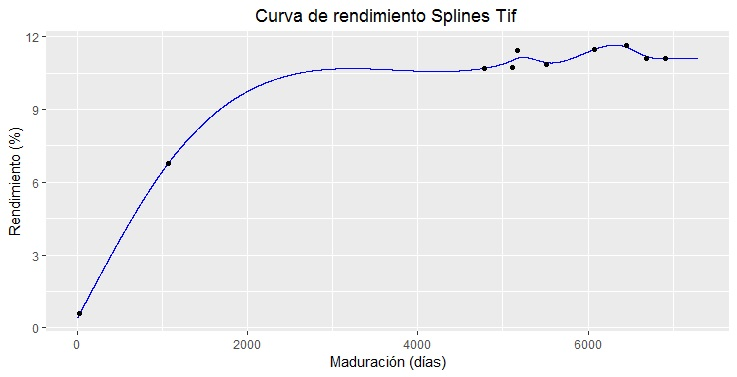
\includegraphics{images/c_tif.jpg}}
%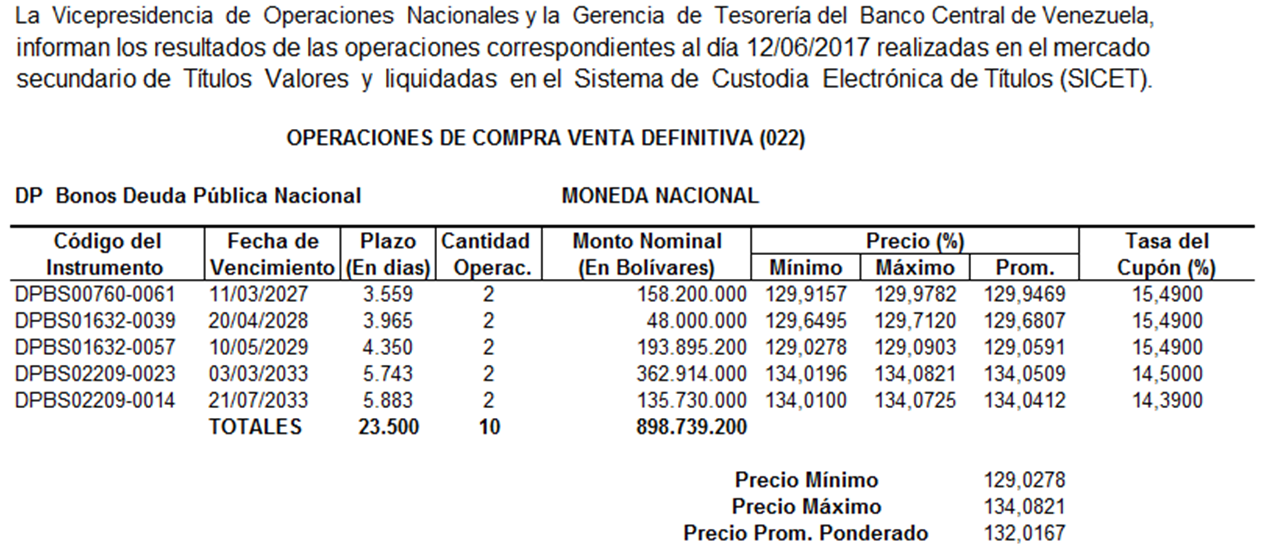
\includegraphics[width=0.7\textwidth]{Imagen022.png}
\caption{Curva Spline TIF.}
\end{figure}

\begin{figure}[h]
  \scalebox{0.80}{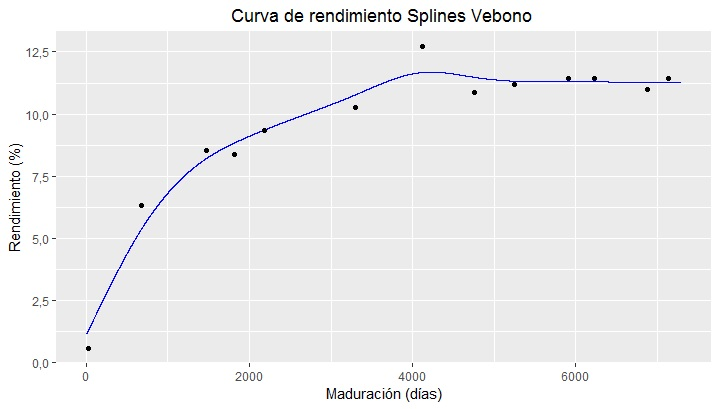
\includegraphics{images/c_veb.jpg}}
%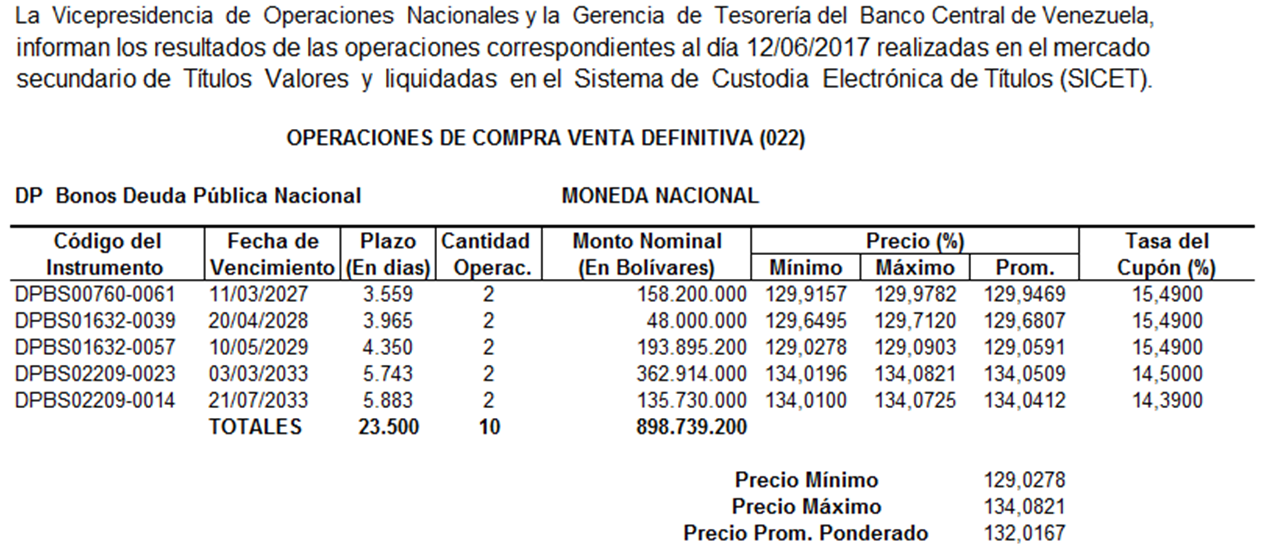
\includegraphics[width=0.7\textwidth]{Imagen022.png}
\caption{Curva Spline VEBONO.}
\end{figure}

\begin{figure}[h]
  \scalebox{0.65}{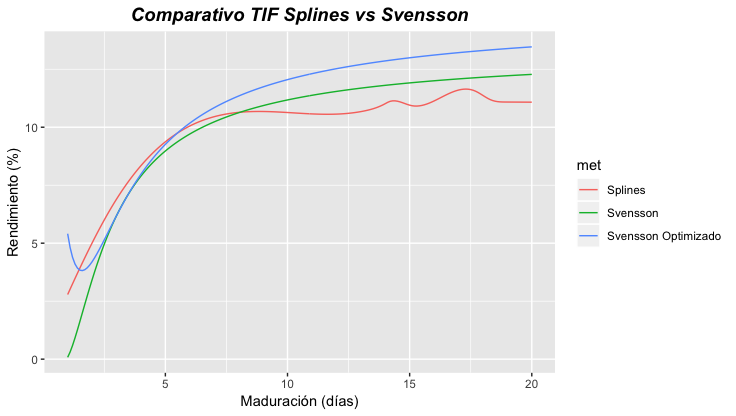
\includegraphics{images/Comparativo_tif.png}}
%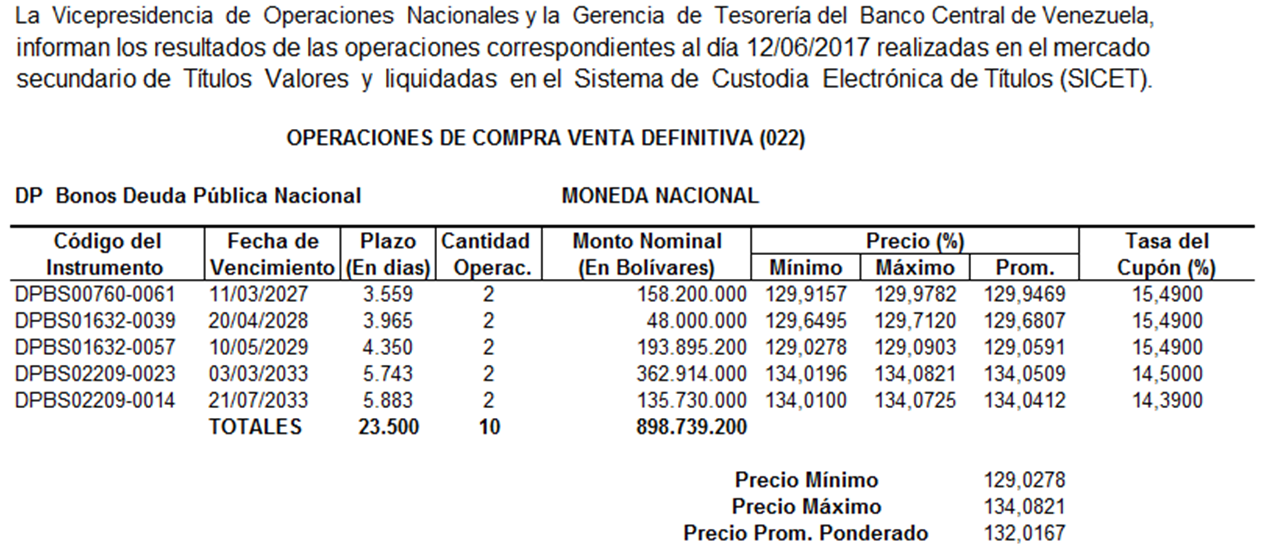
\includegraphics[width=0.7\textwidth]{Imagen022.png}
\caption{Curva TIF Spline vs Svensson.}
\end{figure}

\begin{figure}[h]
  \scalebox{0.65}{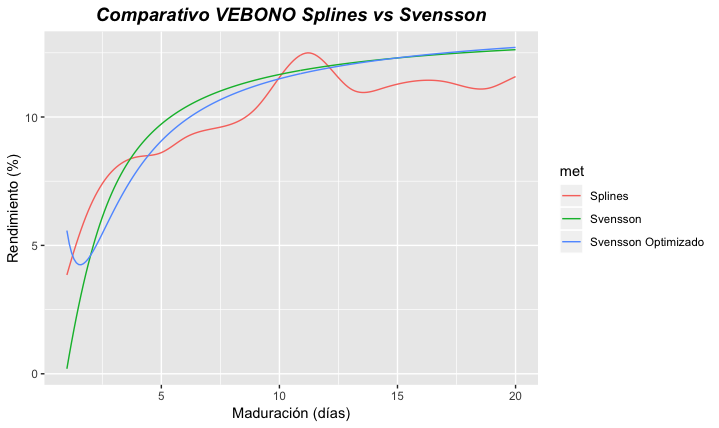
\includegraphics{images/Comparativo_vebono.png}}
%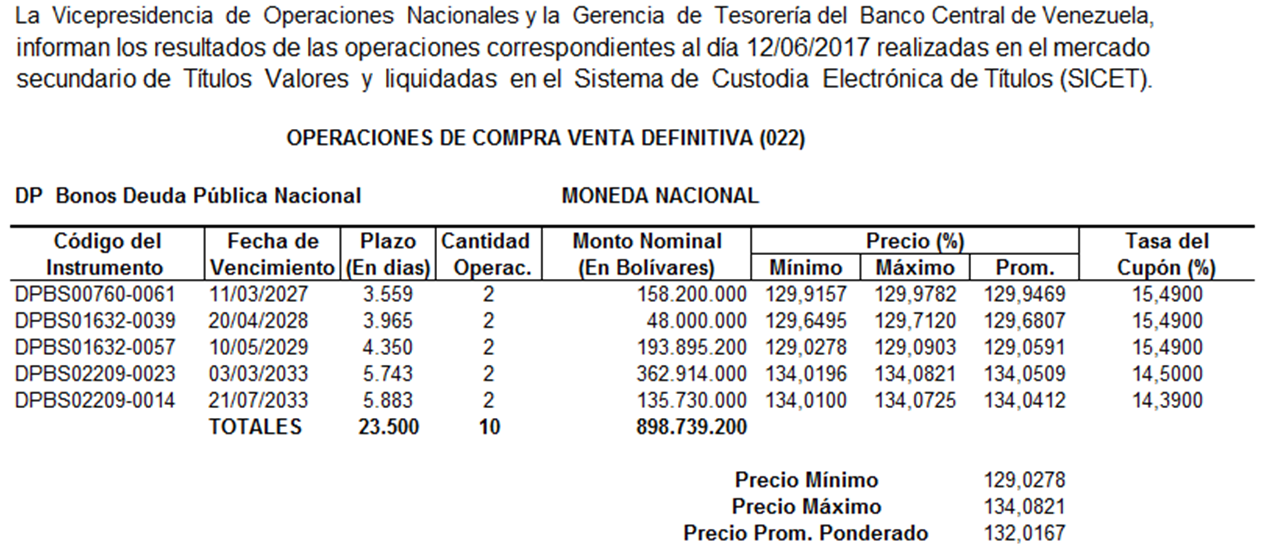
\includegraphics[width=0.7\textwidth]{Imagen022.png}
\caption{Curva VEBONO Spline vs Svensson.}
\end{figure}

\section{Conclusiones y Recomendaciones.}

\hspace{0.4cm}La curva de rendimiento es una herramienta muy importante al momento de obtener informaci\'on acerca de la tasa de inter\'es o rendimiento a una fecha determinada ya que dicha curva relaciona la maduraci\'on o fecha de vencimiento con el rendimiento. Una de las aplicaciones de esta curva, es que a partir de ella es posible obtener con facilidad el precio de un determinado instrumento, bono o t\'itulo, lo cual es de suma utilidad al momento de querer realizar alguna operaci\'on con el mismo, ya sea compra o venta del instrumento, ya que se tendr\'ia de antemano un precio referencial a partir del cual se puede tomar una decisi\'on. En otras palabras, la curva de rendimiento es una herramienta muy \'util al momento de tomar decisiones al realizar alguna inversi\'on.

\vspace{0.5cm}

\hspace{0.4cm} Para determinar dicha curva, varias metodolog\'ias han sido desarrolladas. Existen dos grandes enfoques que permiten su c\'alculo, el primer enfoque se basa en el uso de las metodolog\'ias param\'etricas de estimaci\'on, las cuales se caracterizan por estar atadas a ciertos par\'ametros, su uso es muy frecuete. Entre ellas, principalmente destacan la metodolog\'ia de Nelson y Siegel introducida en 1987 $[2]$, la metodolog\'ia de Svensson desarrollada en 1994 $[3]$, entre otras.

\vspace{0.5cm}

\hspace{0.4cm}Por otra parte, el segundo enfoque se centra en el uso de las metodolog\'ias no param\'etricas, las cuales se caracterizan por su flexibilidad ya que ellas no se encuentran atadas a ning\'un par\'ametro espec\'ifico sino que trabajan directamente con los datos suministrados. Entre ellas, destacan la metodolog\'ia de redes neuronales $[9]$, splines de polinomios $[6]$, splines c\'ubicos suavizados $[7]$, entre otras. En el presenta trabajo se aplica la \'ultima metodolog\'ia mencionada.

\vspace{0.5cm}

\hspace{0.4cm} La principal raz\'on de aplicar la metodolog\'ia de los splines c\'ubicos suavizados, fu\'e el balance que se obtiene como la misma, ya que ella presenta un equilibrio entre el ajuste a los datos y la suavidad de la curva resultante. Lo cual, es \'util cuando la data presenta mucho ruido ya que esta metodolog\'ia no interpola los valores ingresados sino que ajusta una curva suave que presenta el menor error de ajuste posible. En el presente trabajo se emple\'o la data de los Tif y Vebonos, instrumentos de la deuda p\'ublica nacional venezolana para el a\~no 2016 y 2017. Para ambos intrumentos se encontraron una cantidad aceptable de operaciones a partir de las cuales se calcu\'o el rendimiento y as\'i a partir de dichos valores calcular la curva de rendimientos. Una vez obtenida la curva, se procede a estimar los precios de los instrumentos involucrados.
